\maketitle
\tableofcontents
\newpage

\section{Zielsetzung}
Ziel dieses Versuches ist es, gedämpfte und erzwungene Schwingungen zu untersuchen.
Dabei werden auf die Zeitabhängigkeit der gedämpften Schwingung, auf den aperiodischen
Grenzfall und die Frequenzabhängigkeit der Spannung bzw. der Phase zwischen Erreger-
und Kondensatorspannung eingangen.
\section{Theorie}
Ein Schwingkreis besteht in seiner einfachsten Form aus einem Kondensator mit der Kapzität
$C$ und einer Spule mit der Induktivität $L$. Die Energie in diesem Schwingkreis oszilliert
zwischen den beiden Energiespeichern und hat als mögliche Maxima ein maximales magnetisches
Feld in der Spule und einen maximal aufgeladenen Kondensator. Falls ein idealer Draht
vorliegt, wird diese $\textbf{ungedämpfte Schwingung}$ für $t \to \infty$ unverändert schwingen.
\subsection{Gedämpfte Schwingung}
\label{sec:gedaempfteSchwingung}
\begin{figure}
  \centering
  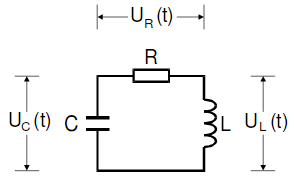
\includegraphics[scale=0.6]{gSchwingkreis.png}
  \caption{Schaltbild eines gedämpften Schwingkreises \cite{anleitung}.}
  \label{fig:1}
\end{figure}

Falls ein endlicher Widerstand $R$ in den Schaltkreis eingebaut wird, siehe \ref{fig:1},
dann wird ein Teil der elektrischen Energie an diesem ohmschen Widerstand in Wärme umgewandelt.
Damit fallen die Amplituden der Spannung und des Stromes mit der Zeit ab und es entwickelt sich
eine $\textbf{gedämpften Schwingung}$. Das Gesetz zwischen Absinken der Amplitude und der Zeit
lässt sich aus dem zweiten Kirchhoffschen Gesetz, mit den Spannungen aus Abbildung \ref{fig:1},
herleiten
\begin{equation}
    U_R (t) + U_L (t) + U_{\symup{C}} (t) = 0 \, .
    \label{eqn:1}
\end{equation}
Daraus wird eine lineare homogene Differentialgleichung 2. Ordnung der Form
\begin{equation}
    \ddot{I}(t) + \frac{R}{L} \ddot{I}(t) +
    \frac{1}{LC} \, I(t) = 0
    \label{eqn:2}
\end{equation}
entwickelt, welche als Lösung
\begin{equation}
  I'(t) = e^{-2 \pi \mu t} \left(A e^{i 2 \pi \nu t} + B e^{-i 2 \pi \nu t}\right)
  \label{eqn:3}
\end{equation}
mit $A$ und $B$ als beliebige Zahlen aus $\mathbb{C}$ und den Abkürzungen
\begin{align}
        2 \pi \mu &= \frac{R}{2L} \\
        \label{eq:1}
        2 \pi \nu &= \sqrt{\frac{1}{LC} - \frac{R^2}{4L^2}}
\end{align}
besitzt. Für den weiteren Verlauf ist es erforderlich zu ermitteln, ob $\nu$
reell oder imaginär ist. Deshalb wird eine Fallunterscheidung ausgeführt:
\begin{itemize}
  \item $\nu$ ist reell:

    Damit in diesem Fall $I'(t)$ reell wird, muss $A = \overline{B}$ gelten. Mit
    geeigneten Ansätzen erhält man schließlich
    \begin{equation}
        I(t) = A_0 \, e^{-2 \pi \mu t} \, \symup{cos} \left(2 \pi f t + \eta \right)
        \label{eqn:4}
    \end{equation}
    mit $A_0$ und $\eta$ als beliebige Zahlen aus $\mathbb{R}$ und $f$ als Frequenz der
    Schwingung. Gleichung \eqref{eqn:4} stellt eine Schwingungsgleichung für eine
    $\textbf{gedämpfte Schwingung}$ dar, deren Amplitude offensichtlich exponentiell gegen 0 strebt.
    Für die Schwingungsdauer ergibt sich
    \begin{equation}
      T = \frac{1}{f} = \frac{2 \pi}{\sqrt{\frac{1}{LC} - \frac{R^2}{4L^2}}} \, .
      \label{eqn:5}
    \end{equation}
    Die Abnahmegeschwindigkeit steckt im Exponenten der e-Funktion in \eqref{eqn:4},
    nämlich im $\mu$. Daraus lässt sich die Abklingdauer $T_\symup{ex}$ definieren
    \begin{equation}
        T_\symup{ex} = \frac{1}{2 \pi \mu} = \frac{2L}{R} \, .
        \label{eqn:6}
    \end{equation}
  \item $\nu$ ist imaginär:

    Gleichung \eqref{eqn:3} besteht nur noch aus vollständig reellen Exponentialfunktionen,
    sodass \eqref{eqn:4} keinen oszillatorischen Anteil besitzt. Dies nennt man
    aperiodische Dämpfung. Abhängig von $A$ und $B$ strebt $I(t)$ monoton gegen 0 oder
    erreicht noch einen Extremwert. Für das Experiment von Bedeutung ist der Spezialfall
    \begin{equation}
        \frac{1}{LC} = \frac{R_{\symup{ap}}^2}{4L^2} \, ,
        \label{eqn:7}
    \end{equation}
    der $\textbf{aperiodischer Grenzfall}$ heißt und für den $f = 0$ ist. Die Amplitude des Stroms strebt maximal schnell
    gegen 0 und besitzt keinen Überschwinger.
\end{itemize}
\subsection{Erzwungene Schwingung}
\begin{figure}
  \centering
  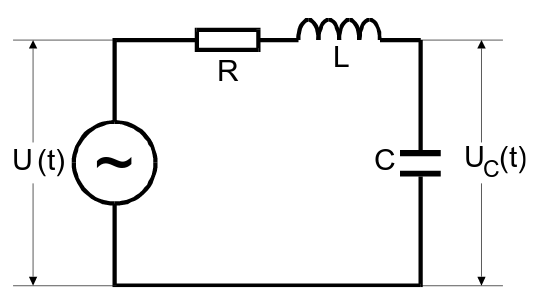
\includegraphics[scale=0.4]{eSchwingkreis.png}
  \caption{Schaltbild einer erzwungenen Schwingung \cite{alt}.}
  \label{fig:2}
\end{figure}
Nun wird der $RCL$-Schwingkreis aus Kapitel \ref{sec:gedaempfteSchwingung} um eine
Wechselstromquelle $U(t)$ erweitert, wie in Abbildung \ref{fig:2} zu sehen. Diese regt den Schwingkreis
sinusförmig mit einer eigenen Frequenz zusätzlich an. Nach einer gewissen Einschwingzeit wird der Schwingkreis
mit derselben Frequenz wie die Wechselstromquelle schwingen.
Mit
\begin{equation*}
    U(t) = U_0 \, e^{i \omega t}
\end{equation*}
wird die Differentialgleichung \eqref{eqn:2} verändert zu
\begin{equation}
    LC \ddot{U}_\symup{C} + RC \ddot{U}_\symup{C} + U_{\symup{C}} = U_0 \, e^{i \omega t} \, .
    \label{eqn:8}
\end{equation}
Um zu ermitteln, wie die Amplitude $U_{\symup{C}_0}$ der Kondensatorspannung mit dem Phasenunterschied
von der Erregerspannung mit der Amplitude $U_0$ und ihrer Frequenz abhängen, nimmt man den Ansatz
\begin{equation*}
  U_{\symup{C}}(\omega, t) = U_{\symup{C}_0}(\omega) \, e^{i \omega t}
\end{equation*}
und setzt ihn in \eqref{eqn:8} ein (Mit $U_{\symup{C}_0}$ als beliebige Zahl aus $\mathbb{C}$). Damit erhält man für die Amplitude
\begin{equation}
    U_{\symup{C}_0} = \frac{U_0 \left(1 -LC \omega^2 - i \omega RC \right)}{\left(1 - LC \omega^2 \right)^2 + \omega^2 R^2 C^2}
    \label{eqn:9}
\end{equation}
und für die Phasenverschiebung $\phi (\omega)$ zwischen $U_{\symup{C}}(t)$ und $U(t)$
\begin{equation}
    \phi (\omega) = \symup{arctan} \left(\frac{-\omega R C}{1 - LC \omega^2}\right) \, .
    \label{eqn:10}
\end{equation}
Mit \eqref{eqn:9} erhält man für die Kondensatorspannung in Abgängigkeit von $\omega$ die sogennante
Resonanzkurve
\begin{equation}
  U_{\symup{C}}(\omega) = \frac{U_0}{\sqrt{\left(1- LC \omega^2\right)^2 + \omega^2 R^2 C^2}} \, .
  \label{eqn:11}
\end{equation}
Für die Frequenzen $\omega_1$ und $\omega_2$ bei denen die Phasenverschiebung genau
$\frac{\pi}{4}$ bzw. $\frac{3\pi}{4}$ beträgt, gilt dann nach \eqref{eqn:10}
\begin{equation}
  \omega_{1,2} = \pm \frac{R}{2L} + \sqrt{\frac{R^2}{4L^2} + \frac{1}{LC}}
  \label{eqn:15}
\end{equation}
An Gleichung \eqref{eqn:11} lässt sich erkennen, dass die Kondensatorspannung für
$\omega \to \infty$ gegen 0 und für $\omega \to 0$ gegen $U_0$ geht. Allerdings
gibt es eine Frequenz, für die die Kondensatorspannung maximiert wird, sodass $U_{\symup{C}} > U_0$ gilt. Dies wird als
Resonanz mit der Resonanzfrequenz
\begin{equation}
  \omega_\symup{res} = \sqrt{\frac{1}{LC} - \frac{R^2}{2L^2}}
  \label{eqn:12}
\end{equation}
bezeichnet. Falls nun die Resonanzfrequenz ungefähr der Frequenz des ungedämpften Schwingkreises
$\omega_0 = \frac{1}{LC}$, d.h. dass in \eqref{eqn:12} $\frac{1}{LC} >> \frac{R^2}{2L^2}$ gilt,
entspricht, so nennt man dies schwache Dämpfung. Für diesen Fall wird $U_{\symup{C}}$ um den Faktor
\begin{equation}
  q = \frac{1}{\omega_0 RC}
  \label{eqn:13}
\end{equation}
größer als $U_0$. \eqref{eqn:13} nennt man auch die $\textbf{Güte q}$ des Schwingkreises.

Eine weitere wichtige Größe ist die Breite der Resonanzkurve aus Formel \eqref{eqn:11}.
Sie wird aus der Differenz der beiden Frequenzen $\omega_+$ und $\omega_-$ gewonnen,
welche sich dadurch auszeichnen, dass $U_{\symup{C}}(\omega_+)$ und $U_{\symup{C}}(\omega_-)$ um den Faktor
$\frac{1}{\sqrt{2}}$ kleiner sind als das Maximum aus \eqref{eqn:13}. Mit der Näherung
\begin{equation*}
  \frac{R^2}{L^2} << \omega_0^2
\end{equation*}
folgt für die Differenz der Frequenzen
\begin{equation}
    \omega_+ - \omega_- \approx \frac{R}{L} \, .
    \label{eqn:14}
\end{equation}

\section{Durchführung}
\subsection{Versuchsaufbau}
\label{sec:versuchsaufbau}
\begin{figure}
  \centering
  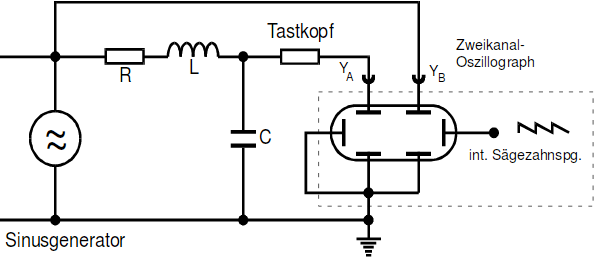
\includegraphics[scale=0.4]{aufbau2.png}
  \caption{Schaltbild des Versuchsaufbaus \cite{anleitung}.}
  \label{fig:3}
\end{figure}
% Wegen dieses Bildes müssen wir nochmal überlegen
\begin{figure}
  \centering
  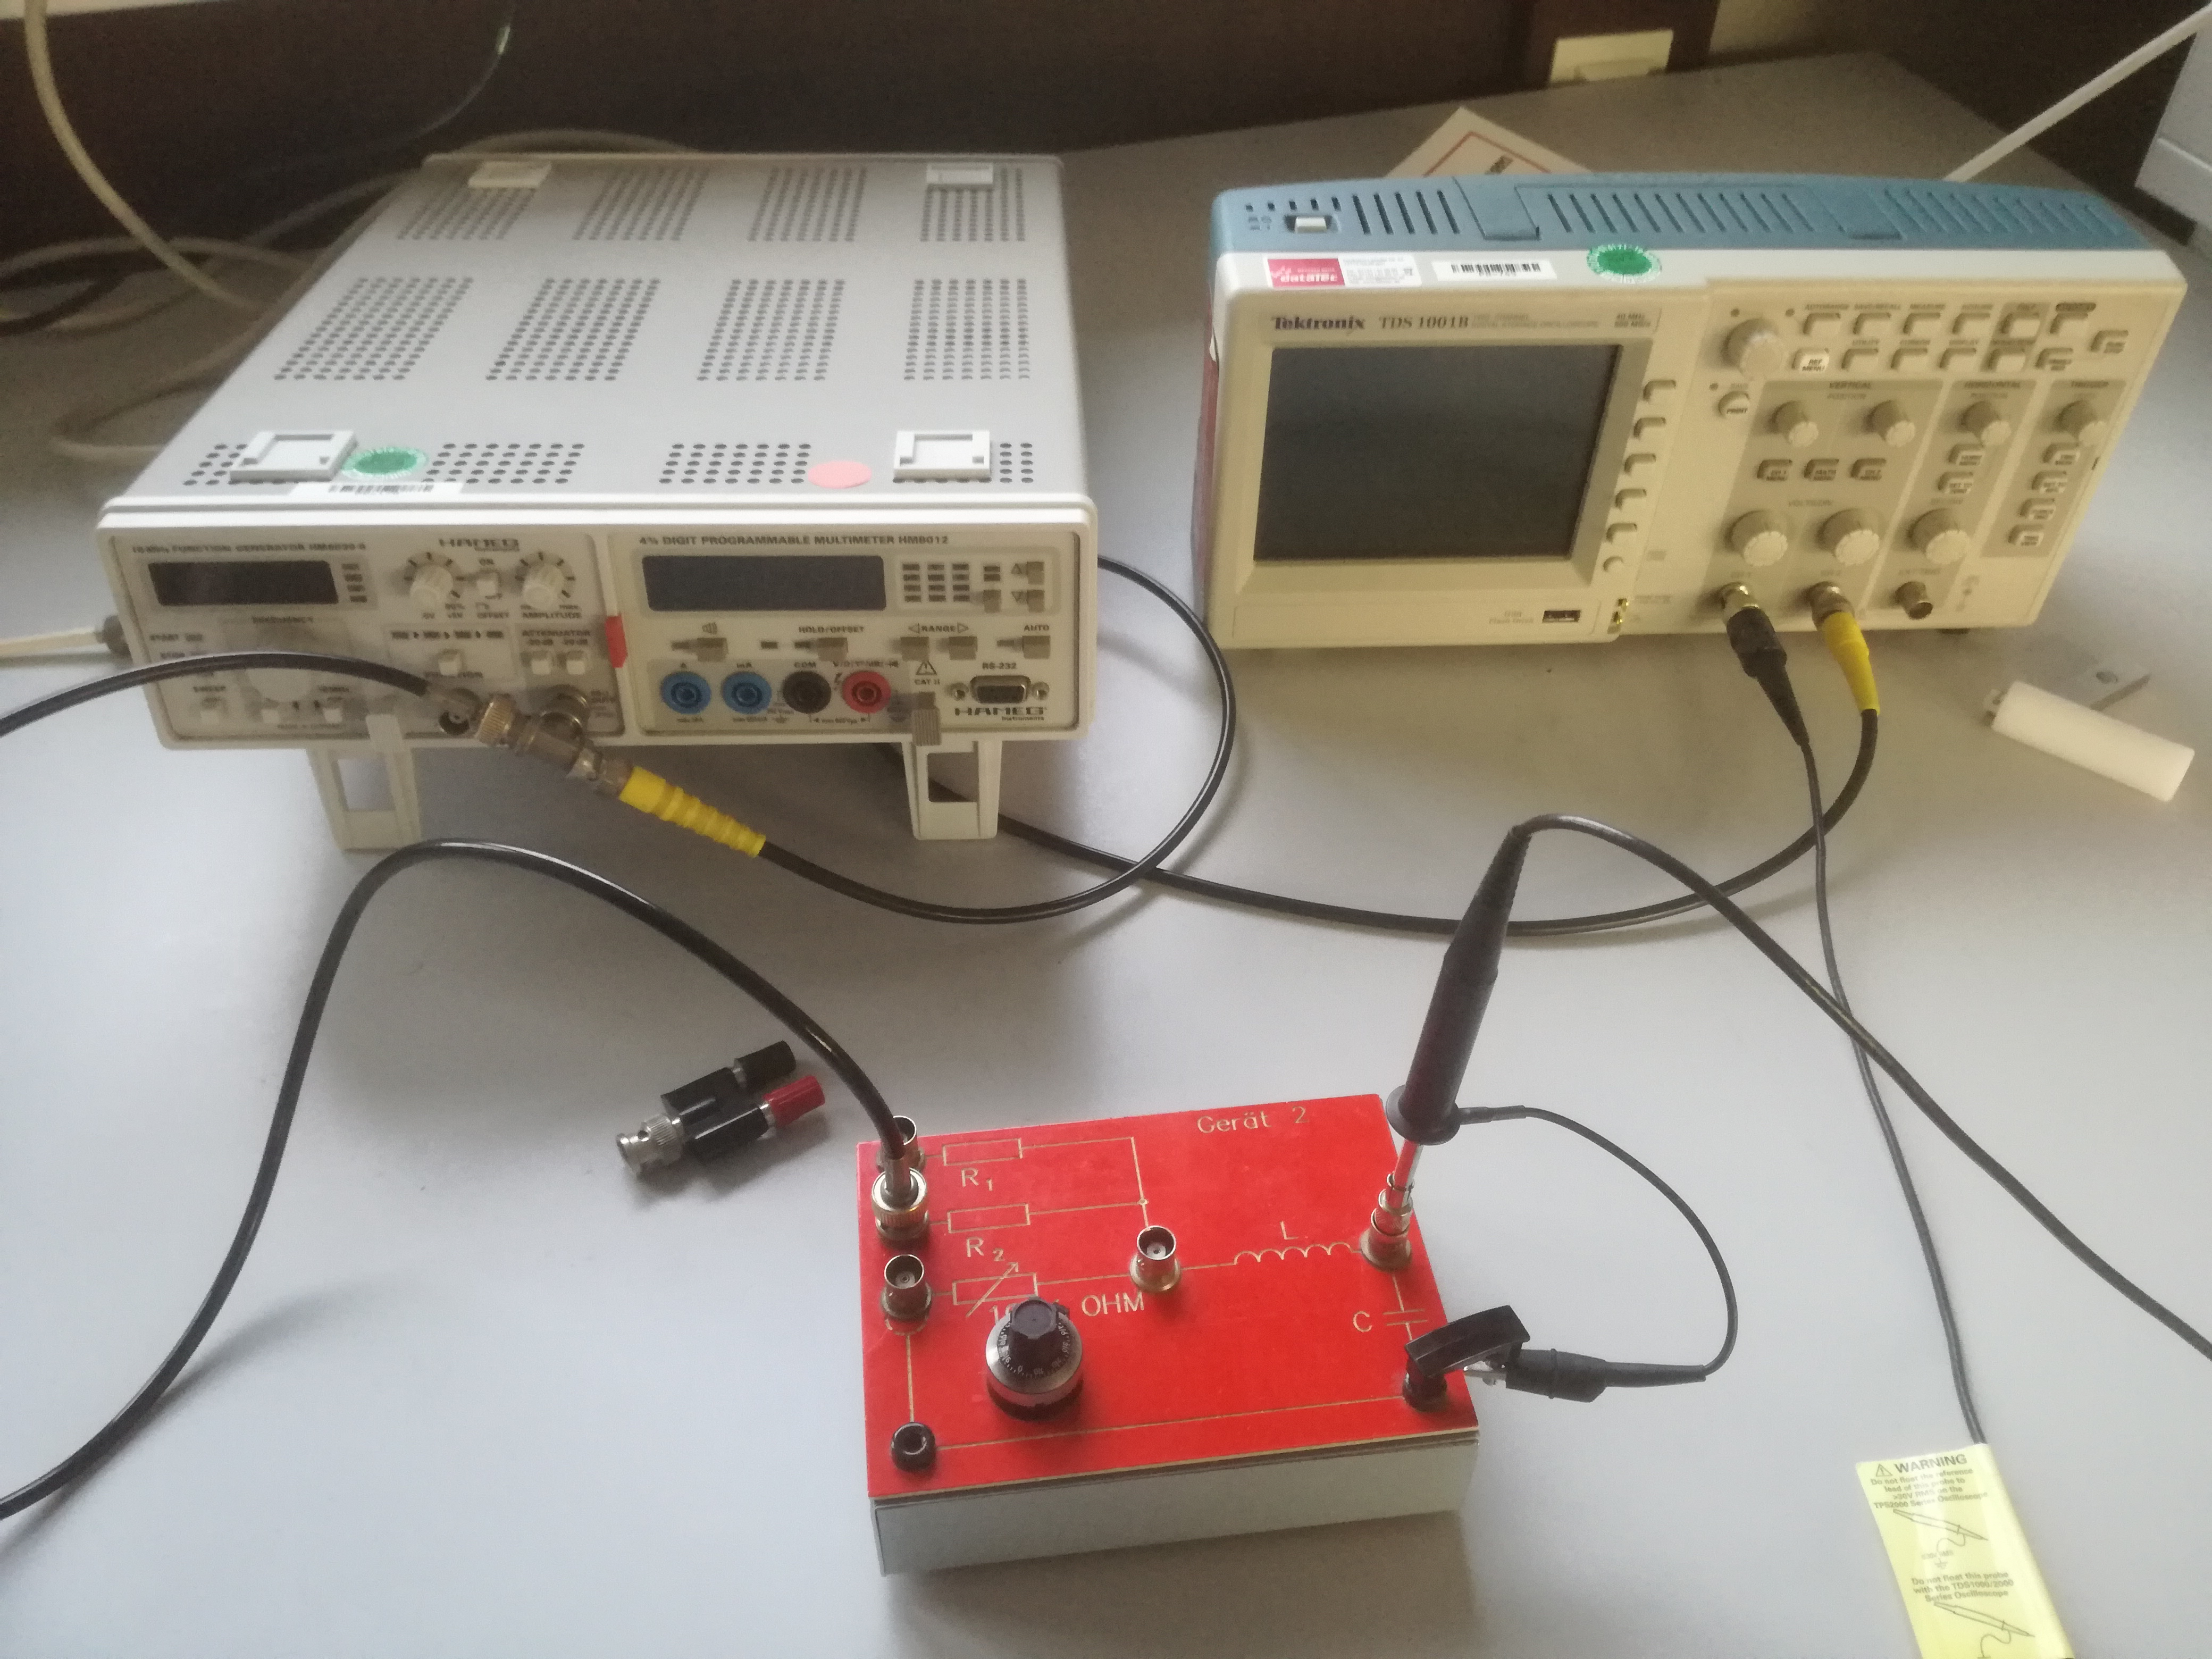
\includegraphics[scale=0.05]{foto.jpg}
  \caption{Foto des Versuchsaufbaus.}
  \label{fig:4}
\end{figure}
Abbildung \ref{fig:3} zeigt einen Sinusgenerator, der nachgeschalteten Schwingkreis
zu Schwingungen anregt. Dazu parallel geschaltet ist ein Oszilloskop, welches über
einen Tastkopf in den Schaltkreis eingebunden wird.

In Abbildung \ref{fig:4} sieht man den Versuchsaufbau im Foto. Der rote Baustein enthält
alle Bestandteile des $RCL$-Schwingkreises plus zwei feste und einen veränderlichen
ohmschen Widerstand. das Gerät auf der linken Seite fungiert als Nadelimpulsgenerator,
kann aber auch die in Kapitel \ref{sec:gedaempfteSchwingung} beschriebene sinusförmige
Spannung liefern. Das rechte Gerät ist ein digitales Oszilloskop, mit dem die Schwingungen
visualisiert werden. Zu diesem Zweck ist der Tastkopf, in Abbildung \ref{fig:3} zu sehen,
in den Schwingkreis eingebaut worden (rechts unten im roten Bauteil steckend).

\subsection{Versuchsdurchführung}
\label{sec:versuchsdurchfuehrung}
Zuerst werden die benötigten Werte über die Widerstände, die Kapazität und die Induktivität
notiert. Dann wird Abbildung \ref{fig:3} aufgebaut, jedoch ohne Verbindung
vom Nadelpulsgenerator zum Oszilloskop und mit dem kleineren der beiden fest eingebauten
ohmschen Widerstände. Dies geschieht, um die Amplitudenabnahme eines
gedämpften Schwingkreises in Abhängigkeit von der Zeit zu ermitteln und daraus
den effektiven Dämpfungswiderstand zu bestimmen. Sodann wird die Spannung gegen die Zeit auf
dem Oszilloskop aufgetragen. Dabei wird darauf geachtet, dass die Amplitude etwa um den Faktor
3 bis 8 abgenommen hat, bevor ein neues Signal des Nadelpulsgenerators eintrifft. Der Schwingungsverlauf
wird mit der Print-Funktion des Oszilloskops festgehalten und ist in Abbildung \ref{fig:5} einsehbar.
\begin{figure}
  \centering
  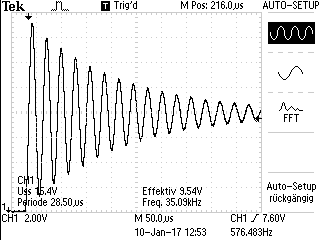
\includegraphics[scale=0.5]{A.png}
  \caption{Schwingsverlauf einer gedämpften Schwingung.}
  \label{fig:5}
\end{figure}
Aus Abbildung \ref{fig:5} wird mit etwa 10 Messpunkten die Amplitudenabnahme und
daraus der effektiven Dämpfungswiderstand bestimmt.

Der Aufbau für die Bestimmung des Dämpunfswiderstandes $R_{\symup{ap}}$, bei dem
der aperiodische Grenzfall eintritt, wird die gleiche Schaltung wie für den ersten Teil der
Durchführung verwendet, mit dem einzigen Unterschied, dass diesmal kein Festwiderstand,
sondern der veränderliche ohmsche Widerstand Teil des Schwingkreises ist. Zunächst
wird der eben erwähnte veränderliche Widerstand auf sein Maximum eingestellt. Auf dem
Oszilloskop äußert sich das durch die monotone Abnahme der Kondensatorspannung, d. h.
es gibt also keine Schwingung. Alsdann wird der Widerstand schrittweise verringert,
bis ein Überschwinger erkennbar wird. Dies bedeutet, dass der Schwingfall eingetreten ist.
Nun wird der Widerstand wieder erhöht, bis dieser Überschwinger verschwunden ist.
\begin{figure}[t]
  \centering
  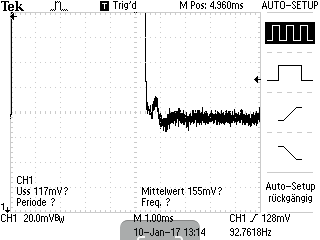
\includegraphics[scale=0.5]{B_nah.png}
  \caption{Spannungsverlauf beim aperiodischen Grenzfall auf einem Oszilloskop.}
  \label{fig:6}
\end{figure}
Dies ist in Abbildung \ref{fig:6} zu sehen. Der eingestellte Widerstand wird als
$R_{\symup{ap}}$ notiert.

Um die Frequenzabhängigkeit der Kondensatorspannung zu untersuchen, wird wieder
die Schaltung aus Kapitel \ref{sec:versuchsaufbau} mit den bereits erwähnten
Änderungen aufgebaut, diesmal mit dem größeren der beiden
Festwiderständ und mit einer Sinusspannung statt Nadelpulsen. Da die Frequenzabhängigkeit
der Phase gleichzeitig ausgeführt wird, wird die Sinusspannung ebenfalls auf dem Oszillsokop
dargestellt. Dann werden beide Spannungsverläufe übereinander gelegt und für elf
verschiedene Frequenzen $U_0$, sprich die Amplitude der Sinusspannung, $U_{\symup{C}}$ und
die zeitliche Differenz zwischen den beiden Nulldurchgängen der Spannungen aufgenommen.
Die Periodenlänge lässt sich aus der jweils eingestellten Frequenz bestimmen.

\section{Auswertung}
Die Daten der in der Apperatur verwendeten Bauteile sind wie folgt:
\begin{align*}
  L &= \SI{10.11(3)}{\milli\henry}\\
  C &= \SI{2.098(6)}{\nano\farad}\\
  R_1 &= \SI{48.1(1)}{\ohm}\\
  R_2 &= \SI{509.5(5)}{\ohm}
\end{align*}
\subsection{Zeitabhängigkeit der gedämpften Schwingung}
\begin{figure}
  \begin{subfigure}{0.74\textwidth}
  \centering
    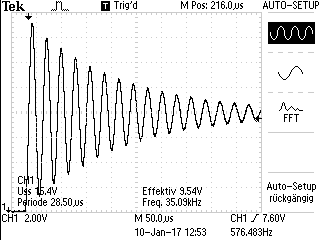
\includegraphics[width=\textwidth]{A.png}
    \qquad
  \end{subfigure}
  \begin{subtable}{0.25\textwidth}
  \centering
  \begin{tabular}{c c}
    \toprule
    $U_{\symup{C}}(t_i)$/\si{\deci\volt} & $t_i$/\si{\micro\second}\\
    \midrule
    7.2 & 40 \\
    6.0 & 70 \\
    5.2 & 100 \\
    4.4 & 130 \\
    3.6 & 160 \\
    3.2 & 180 \\
    2.8 & 210 \\
    2.4 & 240 \\
    2.0 & 270 \\
    1.6 & 300 \\
    \bottomrule
    \end{tabular}
    \qquad
  \end{subtable}
  \caption{In der Tabelle sind die aus dem Oszilloskop-Bild entnommene Datenpaare
  eingetragen. Aufgrund des Verstärkungsfaktors x10 des Tastkopfes sind die Werte
  in \si{\deci\volt} gemessen.}
\label{tab:1}
\end{figure}
Oszilloskop-Bild und daraus entnommenen Wertepaare sind in Abbildung \ref{tab:1}
dargestellt. Durch fitten mit einer Funktion:
\begin{equation}
  U(t)=U_0 \cdot \symup{e}^{-2 \pi \mu t}
\end{equation}
in "curve fit" aus dem Python Paket "scipy optimize" ergeben sich folgende Werte für
$U_0$ und $\mu$:
\begin{align*}
  U_0 &= \SI{0.900(8)}{\volt}\\
  \mu &= \SI[per-mode=reciprocal]{894(12)}{\per\second}
\end{align*}
Aus \eqref{eq:1} und \eqref{eqn:6} folgt dann ein Dämpfungswiderstand $R_{\symup{eff}}$
und eine Abklingzeit $T_{\symup{ex}}$ von:
\begin{align*}
  R_{\symup{eff}} &= \SI{113.6(15)}{\ohm} \\
  T_{\symup{ex}} &= \SI{178(2)}{\micro\second}.
\end{align*}
Im Vergleich mit dem verwendeten Widerstand $\symup{R}_1$ zeigt sich eine Abweichung
von im Mittel \SI{65.5}{\ohm}.

\subsection{Dämpfungswiderstand des aperiodischen Grenzfalls}
Nach \eqref{eqn:7} folgt mit den Bauteilwerten ein rechnerischer Dämpfungswiderstand
\begin{align*}
  R_{\symup{ap}} = \SI{4.39(1)}{\kilo\ohm},
\end{align*}
bei dem der aperiodische Grenzfall eintritt. Gemessen wurde ein Wert von \SI{3.6}{\kilo\ohm}.
Die Abweichung beträgt im Mittel \SI{0.79}{\kilo\ohm}.
\subsection{Frequenzabhängigkeit der Kondensatorspannung}
\begin{table}
  \centering
  \begin{tabular}{c c c c c c c}
    \toprule
    $\nu / \si{\kilo\hertz}$ & $U_{\symup{C}}$/\si{\volt} & $ U_{\symup{err}} / \si{\volt}$
    & $ \frac{U_\symup{C}}{U_{\symup{err}}}$ & $ \symup{\Delta} t / \si{\micro\second}$
    & $T = \frac{1}{\nu} / \si{\nano\second}$
    & $\varphi = \frac{360 \cdot \symup{\Delta}t}{T} / \, \text{deg}$\\
    \midrule
    21 & 1.1 & 0.76 & 1.4 & 1.6 & 47.6 & 12 \\
    25 & 1.4 & 0.74 & 1.9 & 2.4 & 40.0 & 22 \\
    28 & 1.7 & 0.74 & 2.4 & 2.8 & 35.7 & 28 \\
    29 & 1.9 & 0.72 & 2.7 & 3.2 & 34.5 & 33 \\
    30 & 2.1 & 0.72 & 2.9 & 3.4 & 33.3 & 37 \\
    31 & 2.4 & 0.72 & 3.3 & 4.0 & 32.3 & 45 \\
    32 & 2.6 & 0.70 & 3.7 & 5.0 & 31.3 & 58 \\
    33 & 2.7 & 0.70 & 3.9 & 5.8 & 30.3 & 69 \\
    34 & 2.8 & 0.70 & 4.0 & 6.6 & 29.4 & 81 \\
    35 & 2.7 & 0.70 & 3.9 & 7.2 & 28.6 & 91 \\
    36 & 2.5 & 0.70 & 3.7 & 8.4 & 27.8 & 109 \\
    37 & 2.3 & 0.70 & 3.4 & 8.8 & 27.0 & 117 \\
    38 & 2.0 & 0.72 & 2.9 & 9.2 & 26.3 & 126 \\
    39 & 1.8 & 0.72 & 2.5 & 9.4 & 25.6 & 132 \\
    40 & 1.6 & 0.72 & 2.2 & 9.8 & 25.0 & 141 \\
    \bottomrule
    \end{tabular}
    \caption{Messwerte aus den Messungen der Frequenzabhängigkeiten des Schwingkreises.
    Wieder wurde die Kondensatorspannung mit 10-facher Verstärkung gemessen, sodass sie
    in \si{\deci\volt} angegeben wird. Der Wert $\symup{\Delta} t$ gibt den zeitlichen Versatz
    zwischen Kondensator- und Erregerspannung an. Weiterhin finden sich in der Tabelle die
    berechneten Quotienten von Kondensator- und Erregerspannung für Auswertungsteil c), sowie
    die berechneten Periodendauern $T$ und Phasen $\varphi$ für Teil d).}
    \label{tab:2}
\end{table}
Aus den Messwerten in Tabelle \ref{tab:2} folgen die in der selben Tabelle dargestellten
Werte für die Quotienten $ \frac{U_\symup{C}}{U_{\symup{err}}}$. Diese sind in Abbildung
\ref{abb:3} halblogarithmisch sowie linear dargestellt. Beide Graphen liefern die
zu erwartenden Verläufe einer Kurve, die bis zu einem Maximum, der Resonanzfrequenz,
ansteigt und dannach wieder abnimmt.
\begin{figure}
  \centering
  \begin{subfigure}{0.7\textwidth}
  \centering
    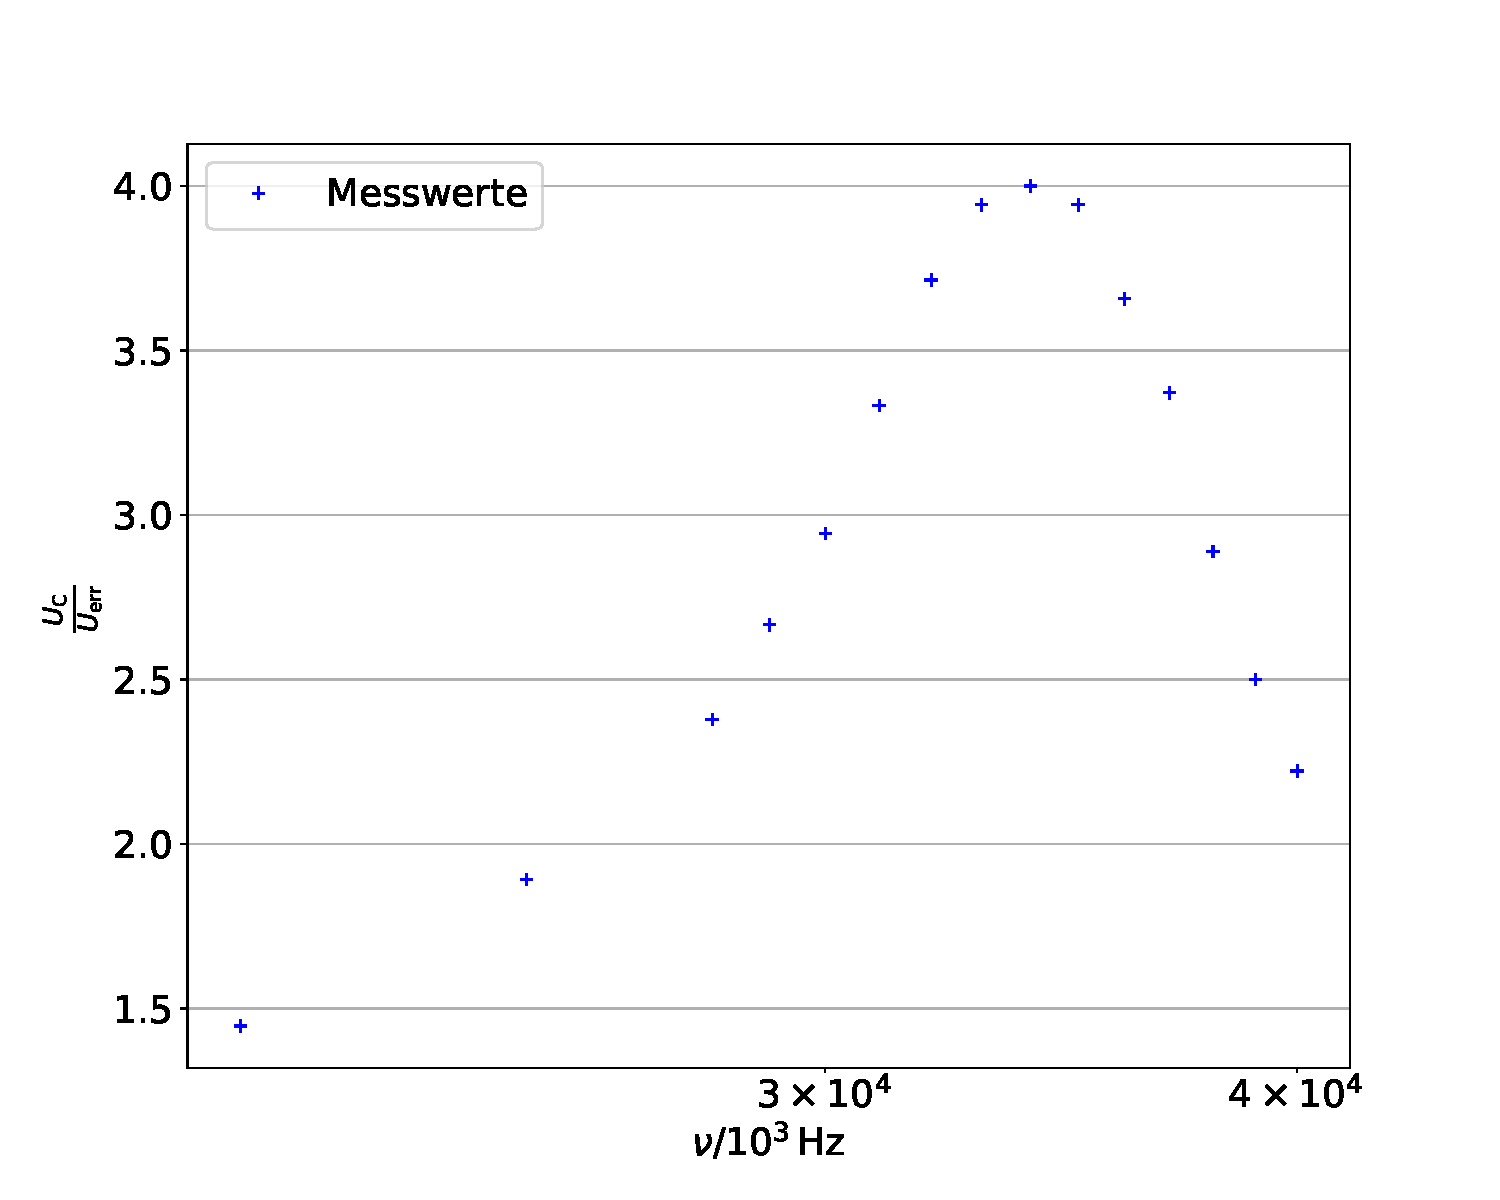
\includegraphics[width=\textwidth]{Halblog.pdf}
    \caption{Halblogarithmische Darstellung.}
    \label{sub:3}
  \end{subfigure}\\
  \begin{subfigure}{0.7\textwidth}
  \centering
    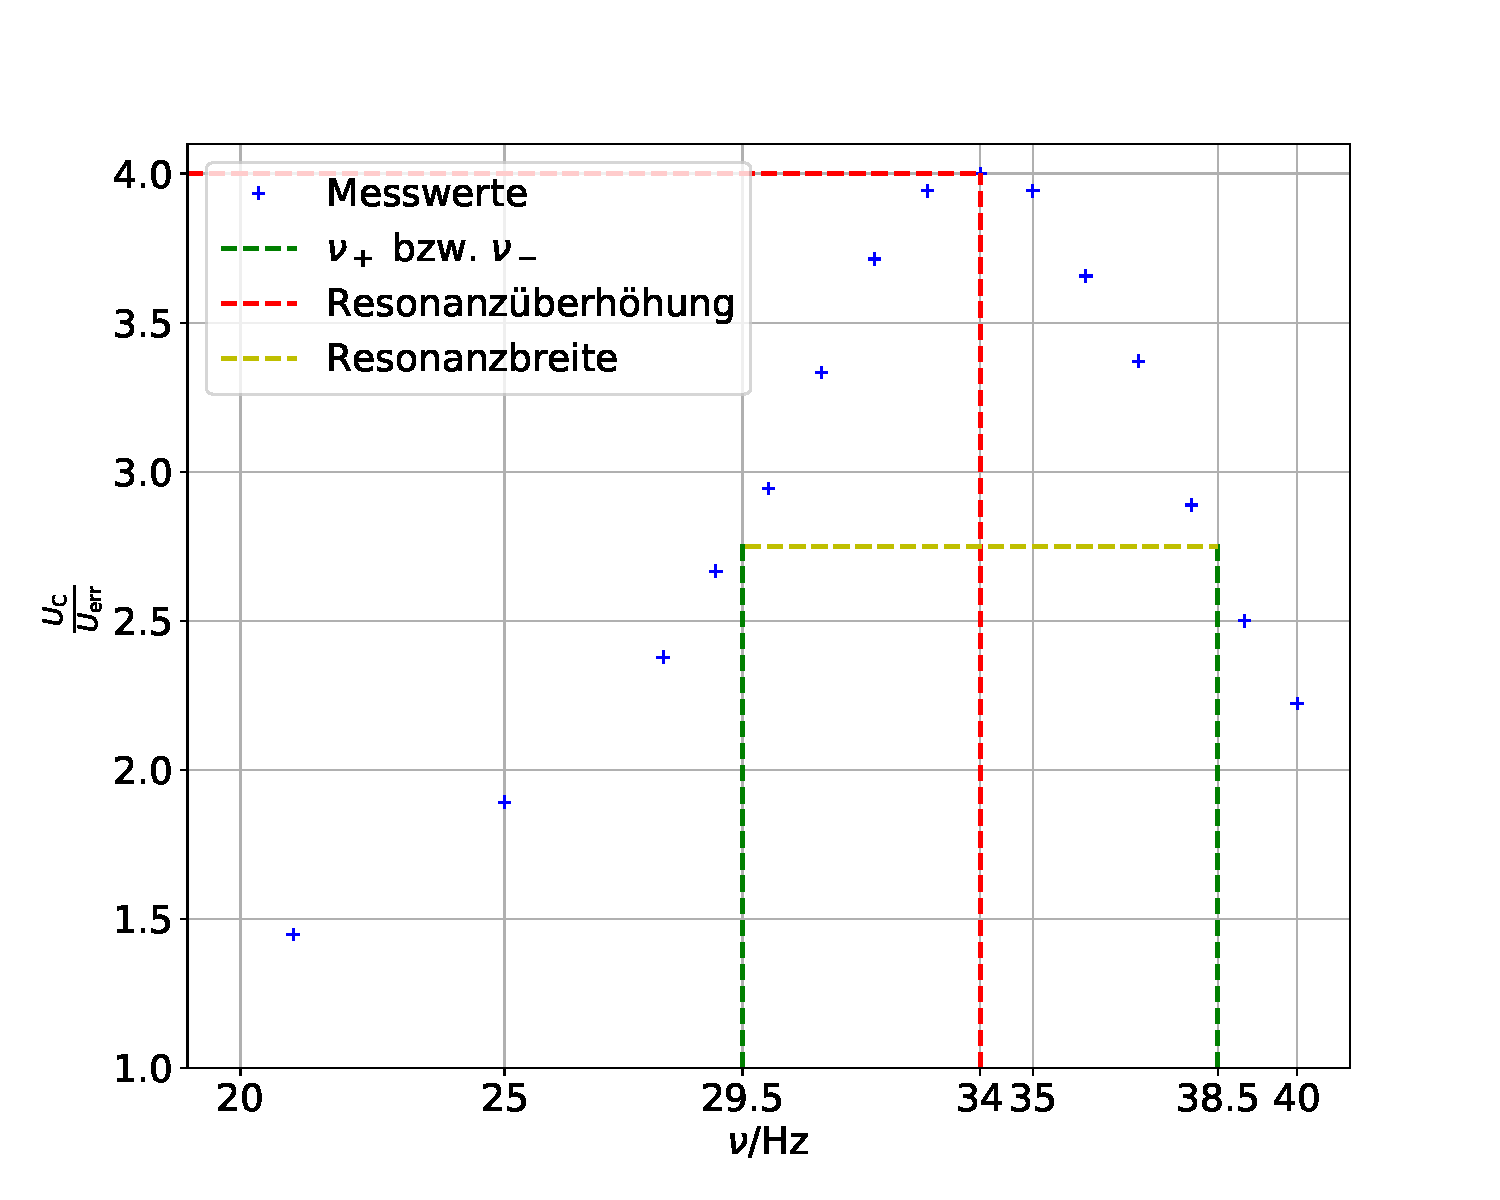
\includegraphics[width=\textwidth]{lin.pdf}
    \caption{Lineare Darstellung mit eingezeichneten Frequenzen.}
    \label{sub:4}
  \end{subfigure}
  \caption{In Abbildung \subref{sub:3} wird der Quotient aus Kondensator- und Erregerspannung gegen die
  Frequenz halblogarithmisch abgetragen. Die gleichen Werte sind in Abbildung \subref{sub:4} linear dargestellt. Hier wurden
  zusätzlich die Resonazfrequenz sowie die Frequenzen $\nu_+$ und $\nu_-$ eingetragen,
  welche die Resonanzkurve begrenzen.}
\label{abb:3}
\end{figure}
Es ergeben sich mit \eqref{eqn:13} und \eqref{eqn:14} die theoretischen Werte für die
Resonanzüberhöhung $q$ sowie die Resonanzbreite $\nu_+ - \nu_-$ sowie aus dem
Diagramm die experimentellen, die mit ihren relativen Abweichungen zueinander in Tabelle \ref{tab:10}
dargestellt sind. In keinem Fall liegt die Abweichung im Rahmen der Fehlertoleranz.
\begin{table}
  \centering
  \begin{tabular}{c c c c}
    \toprule
    & experimentell & rechnerisch  & realtive Abweichung$/ \si{\percent}$\\
    \midrule
    $q$ & \num{4} & \num{4.31(1)} & \num{7.2} \\
    $\nu_+ - \nu_- / \si{\kilo\hertz}$ & \num{9} & \num{8.02(3)} & \num{10.9} \\
    \bottomrule
    \end{tabular}
    \caption{Für $q$ sowie $ \nu_+ - \nu_-$ aus dem Experiment bestimmte
    und errechnete Werte. Zusätzlich ist die relative Abweichung der Werte zueinander
    angegeben.}
    \label{tab:10}
\end{table}
\subsection{Frequenzabhängigkeit der Phase zwischen Erreger- und Kondensatorspannung}
\begin{figure}
  \centering
  \begin{subfigure}{0.7\textwidth}
  \centering
    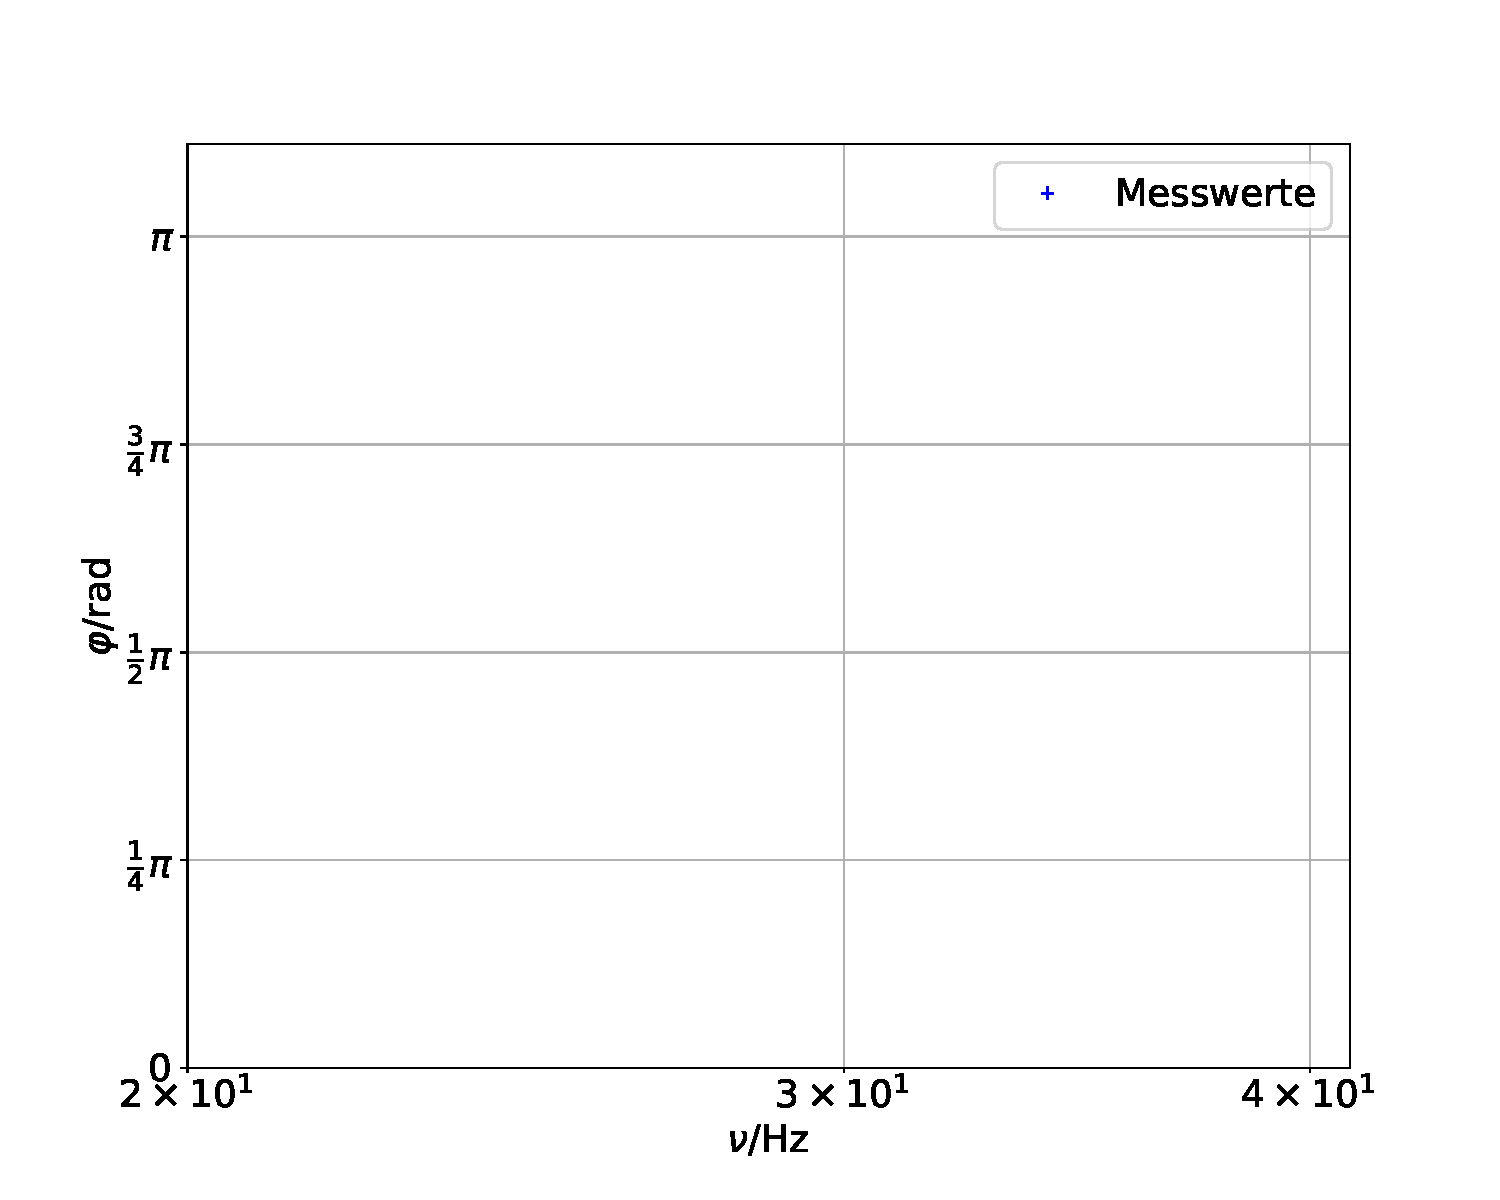
\includegraphics[width=\textwidth]{Phasehalblog.pdf}
    \caption{Halblogarithmische Darstellung.}
    \label{sub:1}
  \end{subfigure}\\
  \begin{subfigure}{0.7\textwidth}
  \centering
    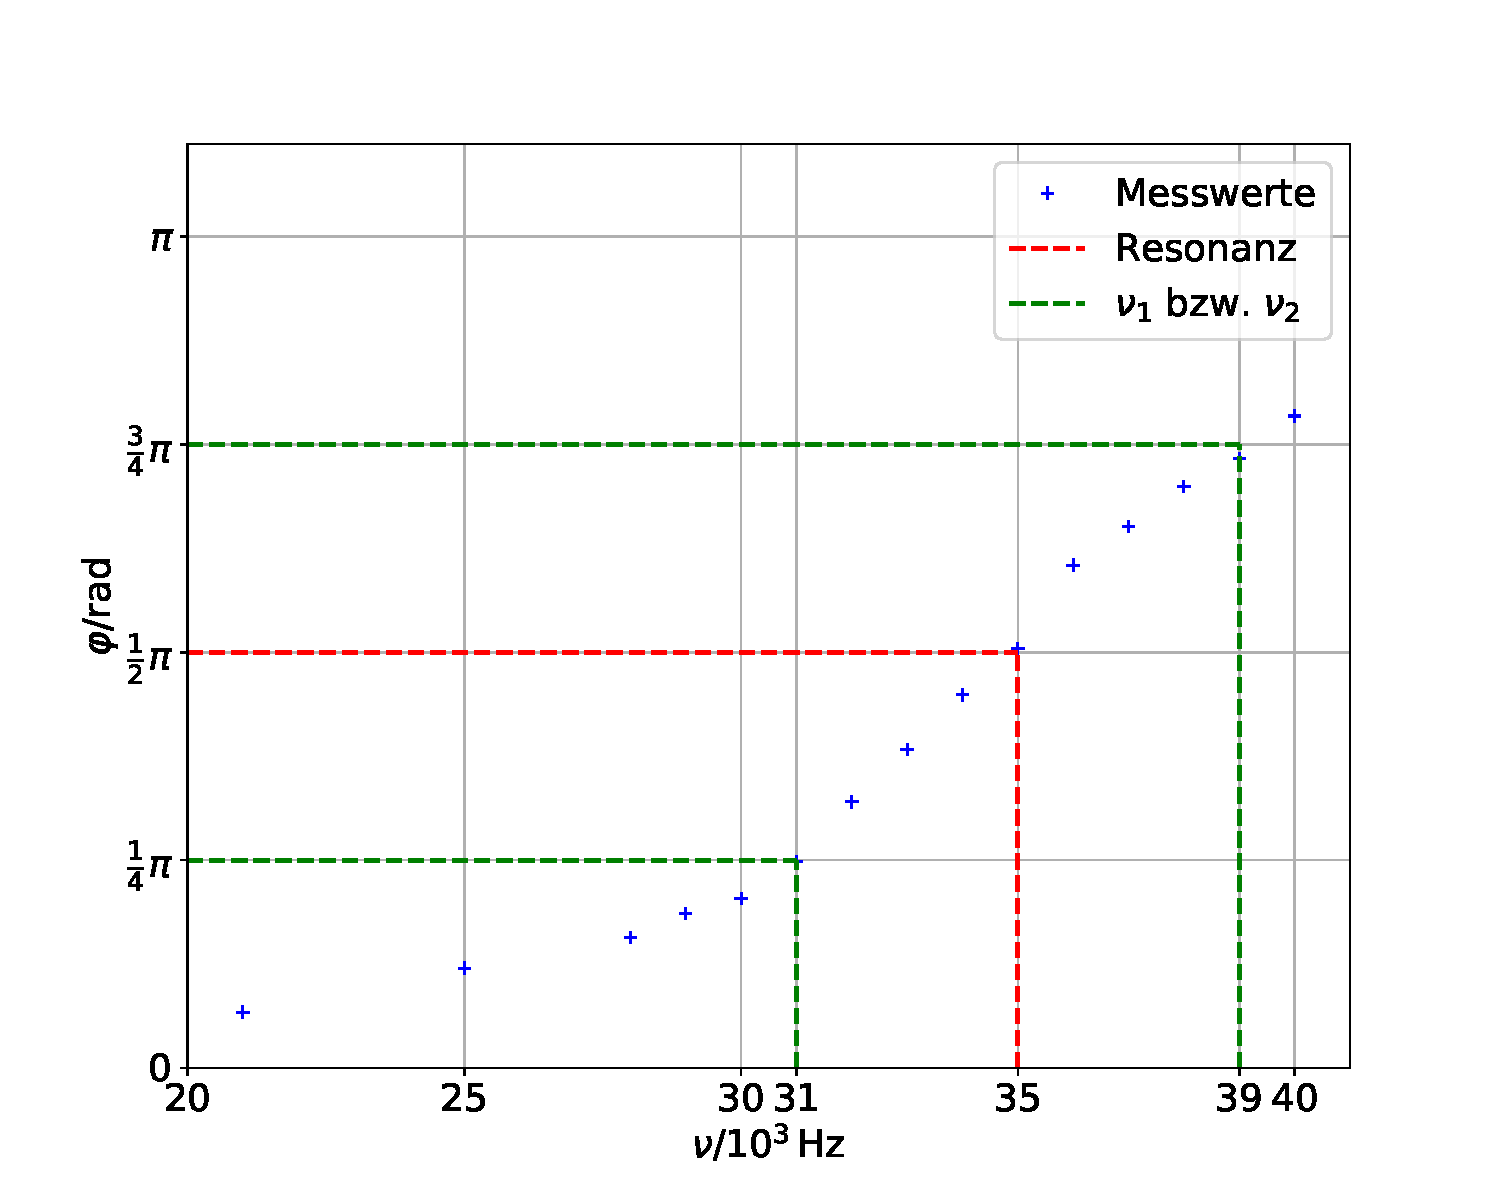
\includegraphics[width=\textwidth]{Phaselin.pdf}
    \caption{Lineare Darstellung.}
    \label{sub:2}
  \end{subfigure}
  \caption{In Abbildung \subref{sub:1} wurden Phase und Frequenz halblogarithmisch gegeneinander
  abgetragen. Die gleichen Werte sind in Abbildung \subref{sub:2} linear dargestellt. Hier wurden
  zusätzlich die Resonazfrequenz sowie die Frequenzen $\nu_1$ und $\nu_2$, also die,
  bei denen eine Phasenverschiebung von $\frac{\pi}{2}$ bzw. $\frac{3 \pi}{2}$ auftritt,
  eingezeichnet.}
\label{abb:2}
\end{figure}
Die gemessenen Werte sind wie oben in Tabelle \ref{tab:2} dargestellt. Tabelle \ref{tab:2}
zeigt ebenfalls die nach
\begin{equation}
  \varphi = \frac{\symup{\Delta}t}{T}
\end{equation}
bestimmten Phasen für die einzelnen Frequenzen. In Abbildung
\ref{abb:2} ist der Verlauf der Phasenverschiebung in Abhängigkeit von der Frequenz
der Erregerspannung aufgetragen. \ref{sub:1} ist dabei in halblogarithmischer
Darstellung. Es zeigt sich der zu erwartende Verlauf der Phasenverschiebung.
Grafik \ref{sub:2} wurde in linearer Darstellung belassen, um ein Ablesen der Frequenzen
zu erleichtern. Die abgelesenen Werte sind zusammen mit den aus \eqref{eqn:15}
für die Frequenzen $\nu_1$ und $\nu_2$ bei $\frac{\pi}{4}$ bzw. $\frac{3 \pi}{4}$
und \eqref{eqn:12} für die Resonanzfrequenz $ \nu_{\symup{res}}$ in Tabelle \ref{tab:3} dargestellt.
Es treten mit unter \SI{3}{\percent} nur geringe relative Abweichen zwischen Theorie und Experiment auf.
Die experimentellen Daten liegen jedoch in keinem Fall im Bereich der Fehlertoleranz
der Theoriewerte.
\begin{table}
  \centering
  \begin{tabular}{c c c c}
    \toprule
    & experimentell & rechnerisch  & realtive Abweichung$/ \si{\percent}$\\
    \midrule
    $\nu_1 / \si{\kilo\hertz}$ & \num{31} & \num{30.78(6)} & \num{0.65} \\
    $\nu_{\symup{res}} / \si{\kilo\hertz}$ & \num{35} & \num{34.09(7)} & \num{2.57} \\
    $\nu_2 / \si{\kilo\hertz}$ & \num{39} & \num{38.80(8)} & \num{0.51} \\
    \bottomrule
    \end{tabular}
    \caption{Für $\nu_1$, $\nu_2$ sowie $ \nu_{\symup{res}}$ aus dem Experiment bestimmte
    und errechnete Werte. Zusätzlich ist die relative Abweichung der Werte zueinander
    angegeben.}
    \label{tab:3}
\end{table}
\section{Diskussion}
\begin{table}
  \centering
  \begin{tabular}{c c c c c}
    \toprule
    Auswertungsteil & Messgröße & experimentell & rechnerisch  & realtive Abweichung$/ \si{\percent}$\\
    \midrule
    a) & $R_{\symup{eff}} / \si{\ohm}$ & \num{48.1(1)} & \num{113.6(15)} & \num{57.7} \\
    \midrule
    b) & $R_\symup{ap} / \si{\kilo\ohm}$ & \num{3.6} & \num{4.39(1)} & \num{18}\\
    \midrule
    c) & $q$ & \num{4} & \num{4.31(1)} & \num{7.2} \\
    & $\nu_+ - \nu_- / \si{\kilo\hertz}$ & \num{9} & \num{8.02(3)} & \num{10.9} \\
    \midrule
    d) & $\nu_1 / \si{\kilo\hertz}$ & \num{31} & \num{30.78(6)} & \num{0.65} \\
    & $\nu_{\symup{res}} / \si{\kilo\hertz}$ & \num{35} & \num{34.09(7)} & \num{2.57} \\
    & $\nu_2 / \si{\kilo\hertz}$ & \num{39} & \num{38.80(8)} & \num{0.51} \\
    \bottomrule
    \end{tabular}
    \caption{Zusammenfassung der Ergebnisse.}
    \label{tab:6}
\end{table}
Die Ergebnisse sind in Tabelle \ref{tab:6} zusammengefasst. Die hohen Abweichungen in
den Teilen a) und b) lassen sich jeweils durch nicht betrachtete Widerstände, insbesondere
dem des Generators, sowie, im Fall von b), durch
die begrenzte maximale Auflösung des Oszilloskopes sowie die Ungenauigkeit des regelbaren Widerstandes erklären.
Zur Verbesserung der Messergebnisse bietet sich die Verwendung von genaueren Geräten
sowie ein genaues Durchmessen der einzelnen Schaltelemente an, um die jeweiligen Widerstände zu bestimmen. Durch konsequentes
beachten dieser Widerstände in den Rechnungen, ließe sich diese systematische Fehlerquelle,
die sich auch auf die nachfolgenden Auswertungsteile auswirkt, ausschließen.\\
Die enormen Abweichungen bei der Bestimmung der Resonanzüberhöhung, also der Güte des Schwingkreises,
lassen sich nur durch fehlerhafte Geräte oder grobe Messfehler erklären. Hier ist
eine weitere Messung notwendig, um die Fehlerquelle zu finden oder zumindest zu
beseitigen. Die Abweichung zwischen dem rechnerisch und dem experimentell bestimmten
Wert für die Breite der Resonanzkurve lässt sich durch die Art der Bestimmung der Werte erklären.
Die graphische Auswertung erfordert Abschätzungen und begünstigt Fehler. Diese ließen sich
durch die Aufnahme von mehr Messwerten abschwächen, welche die Genauigkeit der Bestimmung erhöhen würden.
Gleiches gilt für die Bestimmung von $\nu_1$ und $\nu_2$, die aber um ein Vielfaches
genauer möglich war. Grund war hier, dass die Phasenverschiebungen von $\frac{\pi}{4}$ und
$\frac{3 \pi}{4}$ durch Zufall relativ genau erreicht wurden.\\
Ebenfalls schwierig gestaltete sich das experimentelle Bestimmen der Resonanzfrequenz. Wie in
der Auswertung ersichtlich, wird die Resonanzüberhöhung bei \SI{34}{\kilo\hertz} erreicht,
die in d) bestimmte Resonanzfrequenz jedoch erst bei \SI{35}{\kilo\hertz}. Diese Abweichung
lässt, wie bereits in b), durch genauere Messgeräte vermindern. Die Kondensatorspannung veränderte sich
bei der Messung in einem gewissen Intervall um ihr Maximum nicht, sodass die wirkliche Resonanzfrequenz
darin zu vermuten ist.\\
Zusammenfassend liefert der Versuch also gemischte Ergebnisse. Geringe prozentuale Abweichungen
im letzten Teil werden von großen Abweichungen in den vorrangehenden Teilen überschattet.
Diese lassen sich in den meisten Fällen logisch erklären. Lediglich in Versuchsteil c)
wäre eine erneute Messung unausweichlich, sollten die Ergebnisse verifiziert werden.
\newpage
\nocite{*}
\printbibliography
